%%%%%%%%%%%%%%%%%%%%%%%%%%%%%%%%%%%%%%%%%
% Short Sectioned Assignment LaTeX Template Version 1.0 (5/5/12)
% This template has been downloaded from: http://www.LaTeXTemplates.com
% Original author:  Frits Wenneker (http://www.howtotex.com)
% License: CC BY-NC-SA 3.0 (http://creativecommons.org/licenses/by-nc-sa/3.0/)
%%%%%%%%%%%%%%%%%%%%%%%%%%%%%%%%%%%%%%%%%

%----------------------------------------------------------------------------------------
%	PACKAGES AND OTHER DOCUMENT CONFIGURATIONS
%----------------------------------------------------------------------------------------

\documentclass[paper=a4, fontsize=11pt]{scrartcl} % A4 paper and 11pt font size

% ---- Entrada y salida de texto -----

\usepackage{hyperref}
\usepackage{listings}
\usepackage{color}
%AÑADIDO DE LA PÁGINA http://stackoverflow.com/questions/3175105/how-to-insert-code-into-a-latex-doc
\definecolor{dkgreen}{rgb}{0,0.6,0}
\definecolor{gray}{rgb}{0.5,0.5,0.5}
\definecolor{mauve}{rgb}{0.58,0,0.82}

\lstset{frame=tb,
	language=Python,
	aboveskip=3mm,
	belowskip=3mm,
	showstringspaces=false,
	columns=flexible,
	basicstyle={\small\ttfamily},
	numbers=none,
	numberstyle=\tiny\color{gray},
	keywordstyle=\color{blue},
	commentstyle=\color{dkgreen},
	stringstyle=\color{mauve},
	breaklines=true,
	breakatwhitespace=true,
	tabsize=3
}
%%%%%%%%%%%%%%%%%%%%%%%%%%%%%%%%%%%%%%%%%%%%%%%%%%%%%%%
\usepackage{varioref}
\usepackage[T1]{fontenc} % Use 8-bit encoding that has 256 glyphs
\usepackage[utf8]{inputenc}
%\usepackage{fourier} % Use the Adobe Utopia font for the document - comment this line to return to the LaTeX default

% ---- Idioma --------

\usepackage[spanish, es-tabla]{babel} % Selecciona el español para palabras introducidas automáticamente, p.ej. "septiembre" en la fecha y especifica que se use la palabra Tabla en vez de Cuadro

% ---- Otros paquetes ----

\usepackage{amsmath,amsfonts,amsthm} % Math packages
%\usepackage{graphics,graphicx, floatrow} %para incluir imágenes y notas en las imágenes
\usepackage{graphics,graphicx, float} %para incluir imágenes y colocarlas

% Para hacer tablas comlejas
%\usepackage{multirow}
%\usepackage{threeparttable}

%\usepackage{sectsty} % Allows customizing section commands
%\allsectionsfont{\centering \normalfont\scshape} % Make all sections centered, the default font and small caps

\usepackage{fancyhdr} % Custom headers and footers
\pagestyle{fancyplain} % Makes all pages in the document conform to the custom headers and footers
\fancyhead{} % No page header - if you want one, create it in the same way as the footers below
\fancyfoot[L]{} % Empty left footer
\fancyfoot[C]{} % Empty center footer
\fancyfoot[R]{\thepage} % Page numbering for right footer
\renewcommand{\headrulewidth}{0pt} % Remove header underlines
\renewcommand{\footrulewidth}{0pt} % Remove footer underlines
\setlength{\headheight}{13.6pt} % Customize the height of the header

\numberwithin{equation}{section} % Number equations within sections (i.e. 1.1, 1.2, 2.1, 2.2 instead of 1, 2, 3, 4)
\numberwithin{figure}{section} % Number figures within sections (i.e. 1.1, 1.2, 2.1, 2.2 instead of 1, 2, 3, 4)
\numberwithin{table}{section} % Number tables within sections (i.e. 1.1, 1.2, 2.1, 2.2 instead of 1, 2, 3, 4)

\setlength\parindent{0pt} % Removes all indentation from paragraphs - comment this line for an assignment with lots of text

\newcommand{\horrule}[1]{\rule{\linewidth}{#1}} % Create horizontal rule command with 1 argument of height


\renewcommand{\reftextbefore}
	{en la  \reftextvario{página que precede a esta}{página anterior}}
\renewcommand{\reftextafter}
	{en la \reftextvario{siguiente}{siguiente} página}
\renewcommand{\reftextfacebefore}
	{en la  \reftextvario{anterior}{anterior} página}
\renewcommand{\reftextfaceafter}
	{en la \reftextvario{siguiente}{siguiente}{página}}

%----------------------------------------------------------------------------------------
%	TÍTULO Y DATOS DEL ALUMNO
%----------------------------------------------------------------------------------------

\title{	
\normalfont \normalsize 
\textsc{{\bf Algorítmica (2015-2016)} \\ Grado en Ingeniería Informática \\ Universidad de Granada} \\ [25pt] % Your university, school and/or department name(s)
\horrule{0.5pt} \\[0.4cm] % Thin top horizontal rule
\huge Práctica 1: Análisis de eficiencia de algoritmos \\ % The assignment title
\horrule{2pt} \\[0.5cm] % Thick bottom horizontal rule
}

\author{Francisco Carrillo Pérez,Borja Cañavate Bordons, \\Miguel Porcel Jiménez,Jose Manuel Rejón Santiago,Jose Arcos Aneas} % Nombre y apellidos

\date{\normalsize\today} % Incluye la fecha actual

%----------------------------------------------------------------------------------------
% DOCUMENTO
%----------------------------------------------------------------------------------------

\begin{document}

\maketitle % Muestra el Título

\newpage %inserta un salto de página

\tableofcontents % para generar el índice de contenidos

\listoffigures

\listoftables

\newpage

\section{Introducción }

El objetivo de ésta práctica es analizar implementar y comparar una solución divide y vencerás.
Para ello, hemos recogido los diferentes tiempos de los diferentes algoritmos que hemos diseñado y los hemos comparado.
En nuestro caso concreto, hemos utilizado la biblioteca de C++ más moderna y precisa destinado a obtener tiempos de reloj: la biblioteca \textbf{chrono}

La máquina que hemos utilizado tiene las siguientes características:
	
\begin{itemize}
		
	\item Procesador: Intel Core i5-3337U (2.7GHz x 2)
	\item Memoria RAM: 4GB
	\item Disco Duro: 500GB 5400 rpm
	\item SO: Manjaro Linux 15.2 Capella 64 bits
\end{itemize}
	



%------------------------------------------------
\section{Fuerza bruta} % Sections can be created in order to organize your presentation into discrete blocks, all sections and subsections are automatically printed in the table of contents as an overview of the talk
%------------------------------------------------


En esta parte hemos diseñado dos algoritmos distintos, el primero es un algoritmo muy ineficiente de fuerza bruta que lo que hará 
\begin{figure}[H]
	\centering
	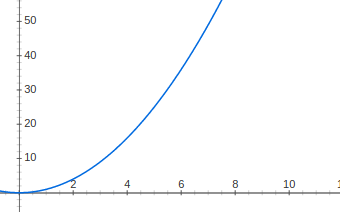
\includegraphics[scale=0.5]{imagenes/enecuadrado.png}
	\caption{Gráfica de la función $n^2$}
	\label{fig:E1}
\end{figure}



\subsection{Burbuja}


La gráfica empírica obtenida ha sido:
\begin{figure}[H]
	\centering
	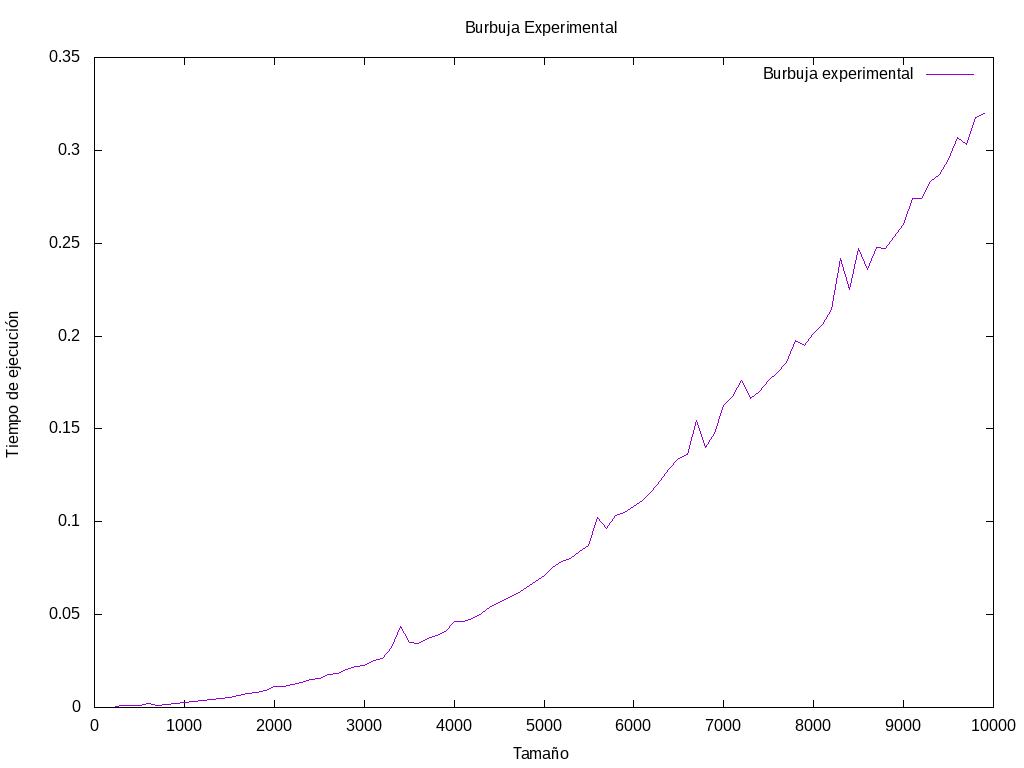
\includegraphics[scale=0.5]{imagenes/burbuja-experimental.png}
	\caption{Algoritmo de Burbuja, gráfica empírica.}
	\label{fig:E2}
\end{figure}





La gráfica híbrida obtenida ha sido:
\begin{figure}[H]
	\centering
	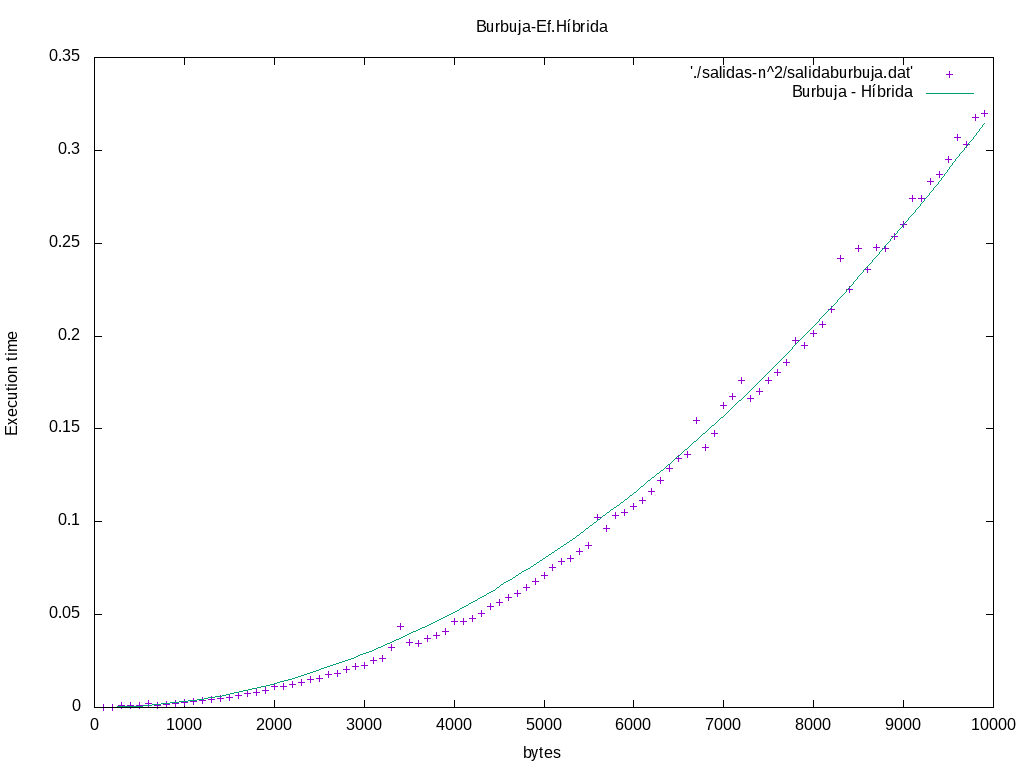
\includegraphics[scale=0.5]{imagenes/burbuja-hibrida.png}
	\caption{Ajuste híbrido algoritmo Burbuja y función $n^2$}
	\label{fig:E3}
\end{figure}	






\subsection{Selección}


La gráfica empírica obtenida ha sido:
\begin{figure}[H]
	\centering
	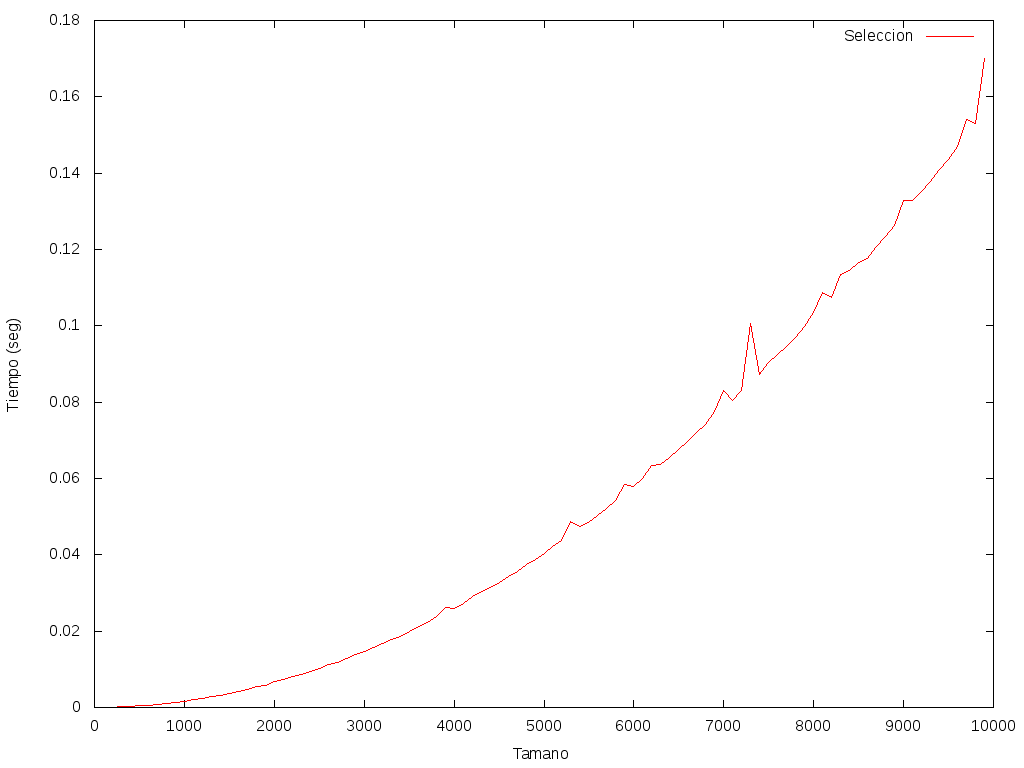
\includegraphics[scale=0.5]{imagenes/seleccionLines.png}
	\caption{Algoritmo de selección, gráfica empírica. }
	\label{fig:E4}
\end{figure}




La gráfica híbrida obtenida ha sido:
\begin{figure}[H]
	\centering
	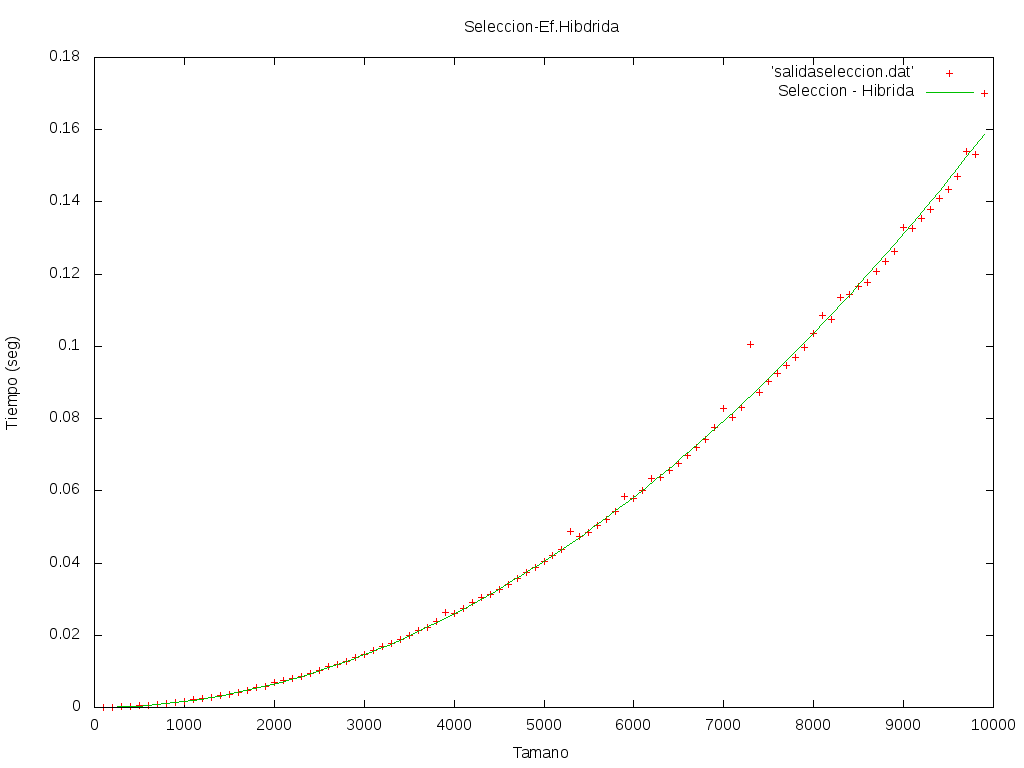
\includegraphics[scale=0.5]{imagenes/seleccion-hibrida.png}
	\caption{Gráfica ajuste híbrido. Selección y $n^2$}
	\label{fig:E5}
\end{figure}


\subsection{Inserción}

La gráfica empírica obtenida ha sido:
\begin{figure}[H]
	\centering
	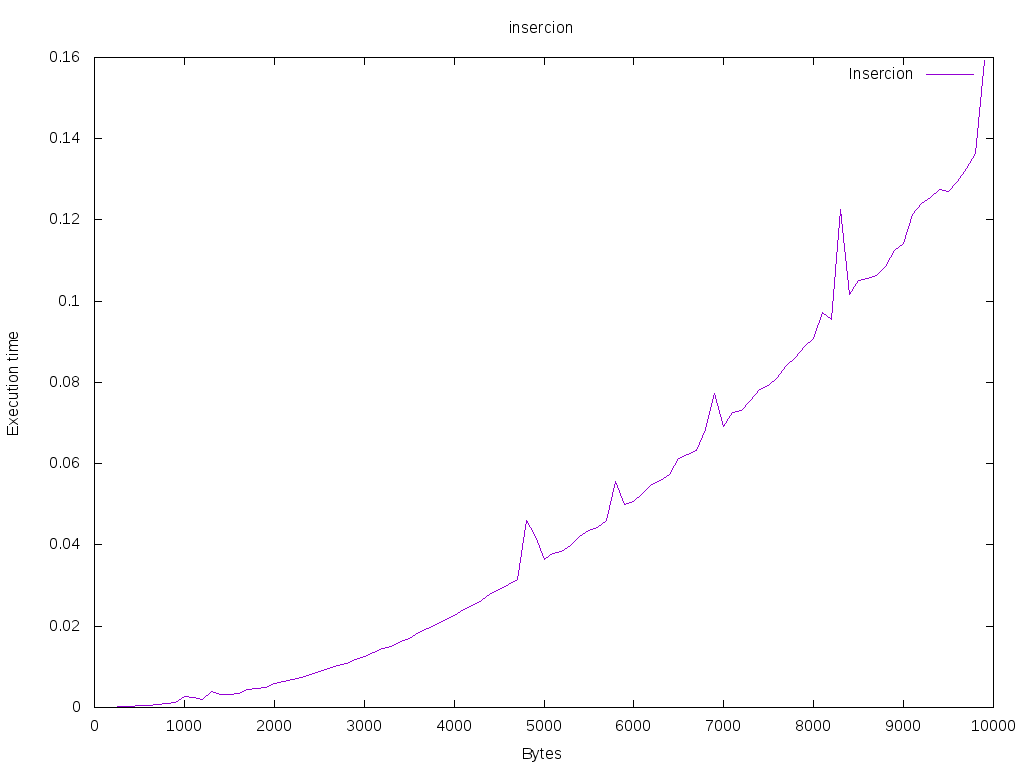
\includegraphics[scale=0.5]{imagenes/insercion.png}
	\caption{Algoritmo de Inserción, gráfica empírica.}
	\label{fig:E6}
\end{figure}


La gráfica híbrida obtenida ha sido:
\begin{figure}[H]
	\centering
	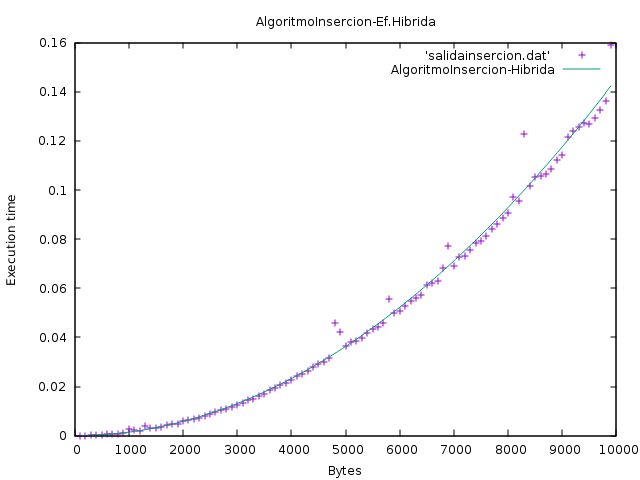
\includegraphics[scale=0.5]{imagenes/algoritmoInsercion-hibrida}
	\caption{Gráfica ajuste híbrido. Inserción y $n^2$}
	\label{fig:E7}
\end{figure}
Por último, mostramos el porcentaje de error así como las constantes ocultas obtenidas.\\
\begin{center}
	\begin{tabular}{| l | c | r |}
		\hline
		\textbf{Algoritmo} & \textbf{Constante Oculta} & \textbf{Error} \\
		\hline
		Burbuja & a0 = 3.20873e-09 & +/- 1.403e-11 (0.4372\%)\\ \hline
		Selección & a0 = 1.61988e-09 & +/- 4.818e-12 (0.2975\%) \\ \hline		
		Inserción & a0 = 1.45151e-09 &  +/- 8.337e-12    (0.5743\%) \\ \hline
	\end{tabular}
\end{center}


\section{Ordenación rápida} % Sections can be crea es muy bajoted in order to organize your presentation into discrete blocks, all sections and subsections are automatically printed in the table of contents as an overview of the talk
%------------------------------------------------
Según hemos ido estudiado, estos algoritmos que presentamos tienen teóricamente y calculando a partir del código una eficiencia de $O(n*\log(n) )$. Como esto es teórico, vamos a ver si efectivamente (o no) los algoritmos proporcionados se parecen a la gráfica de $n*\log(n)$ recogiendo la información de 99 posibilidades distintas en cada algoritmo.
\begin{figure}[H]
	\centering
	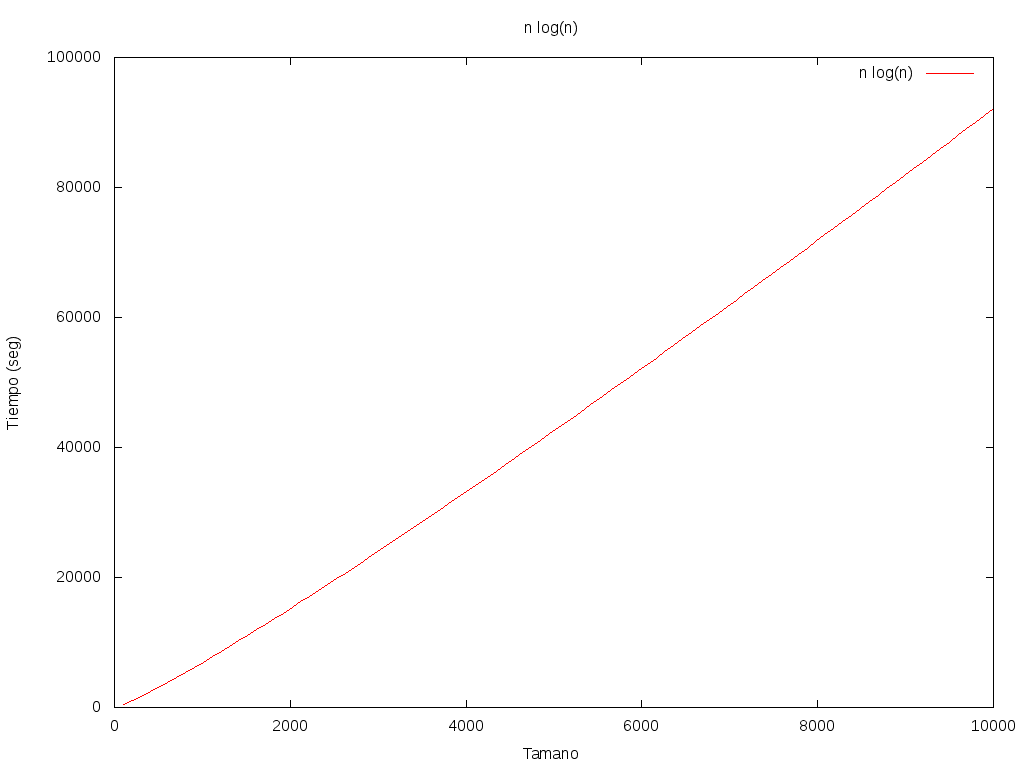
\includegraphics[scale=0.5]{imagenes/nlog(n)3.png}
	\caption{Gráfica de la función $n*log(n)$}
	\label{fig:E8}
\end{figure}
\subsection{Quick Sort}
La gráfica empírica obtenida ha sido:
\begin{figure}[H]
	\centering
	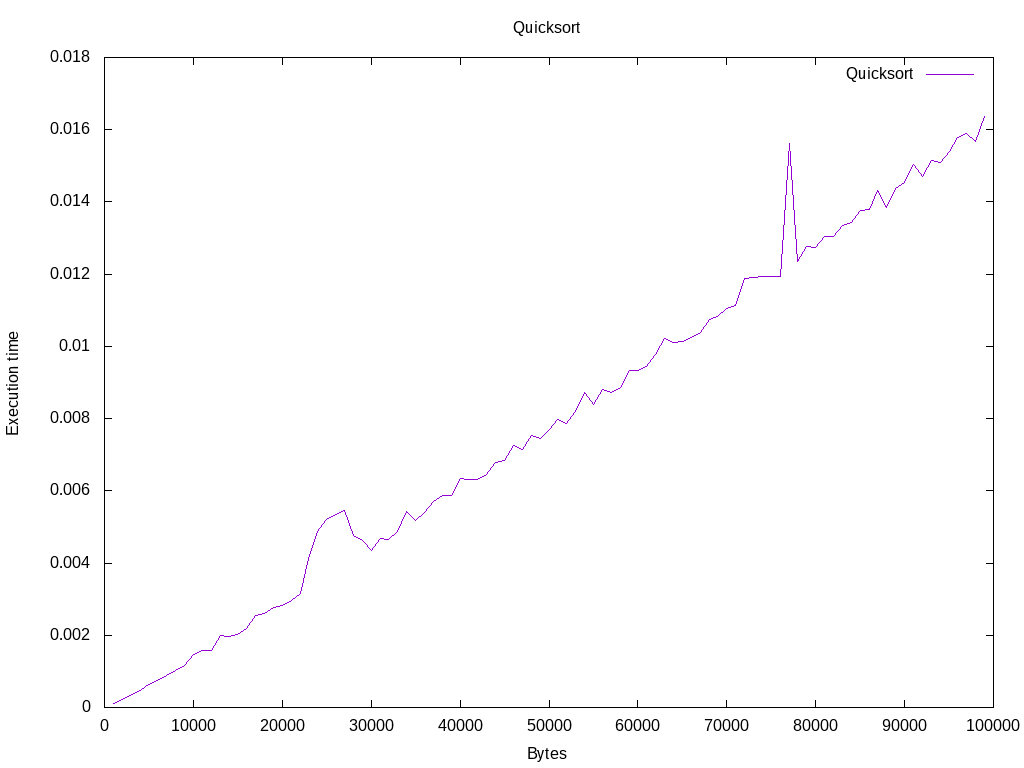
\includegraphics[scale=0.5]{imagenes/quicksort.png}
	\caption{Algoritmo Quicksort, gráfica empírica. }
	\label{fig:E9}
\end{figure}

La gráfica híbrida obtenida ha sido:
\begin{figure}[H]
	\centering
	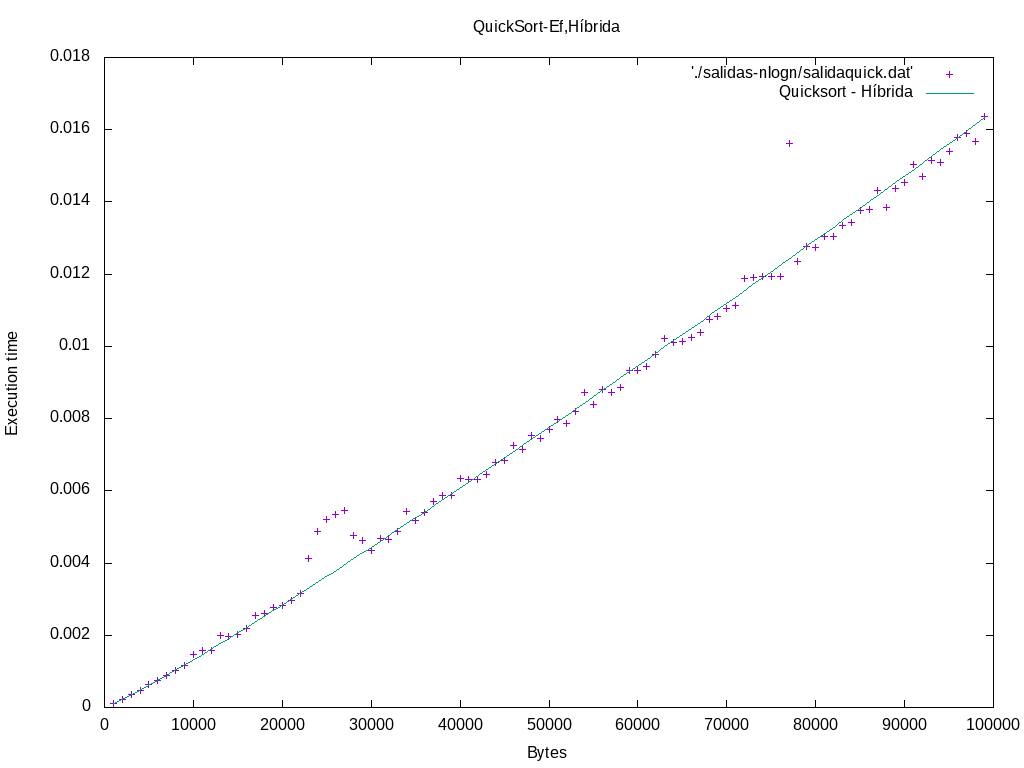
\includegraphics[scale=0.5]{imagenes/quicksort-hibrida.png}
	\caption{Gráfica híbrida Quicksort.}
	\label{fig:E10}
\end{figure}

\subsection{Heap Sort}
La gráfica empírica obtenida ha sido:
\begin{figure}[H]
	\centering
	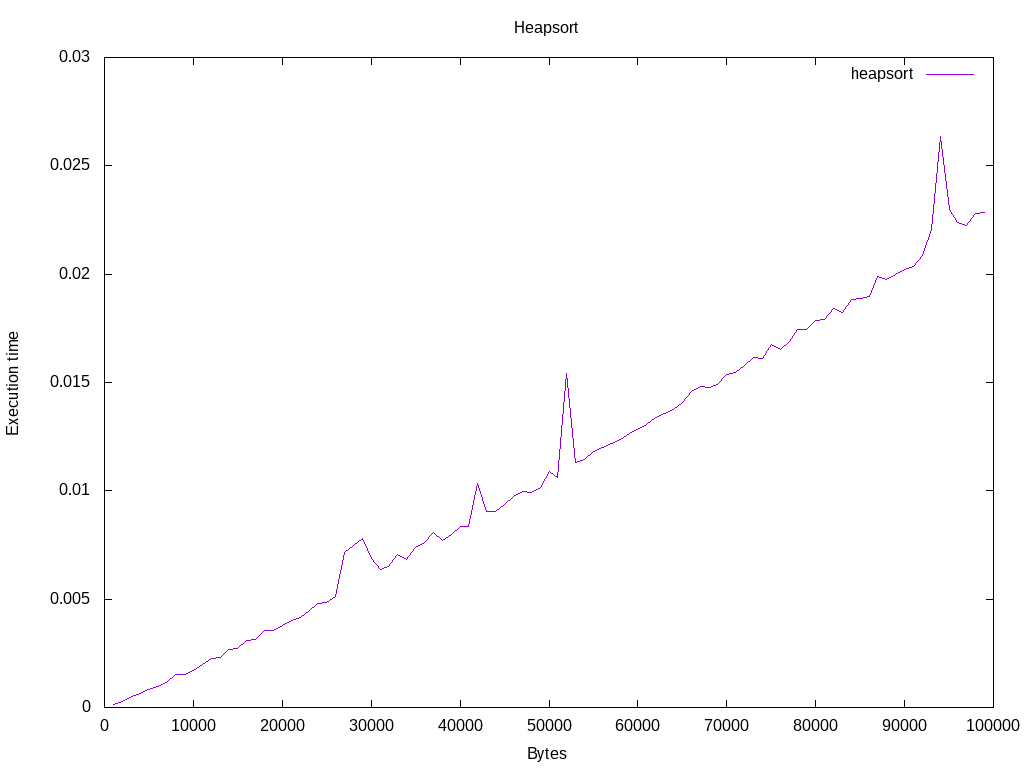
\includegraphics[scale=0.5]{imagenes/heapsort.png}
	\caption{Heapsort, gráfica empírica.}
	\label{fig:E11}
\end{figure}

La gráfica híbrida obtenida ha sido:
\begin{figure}[H]
	\centering
	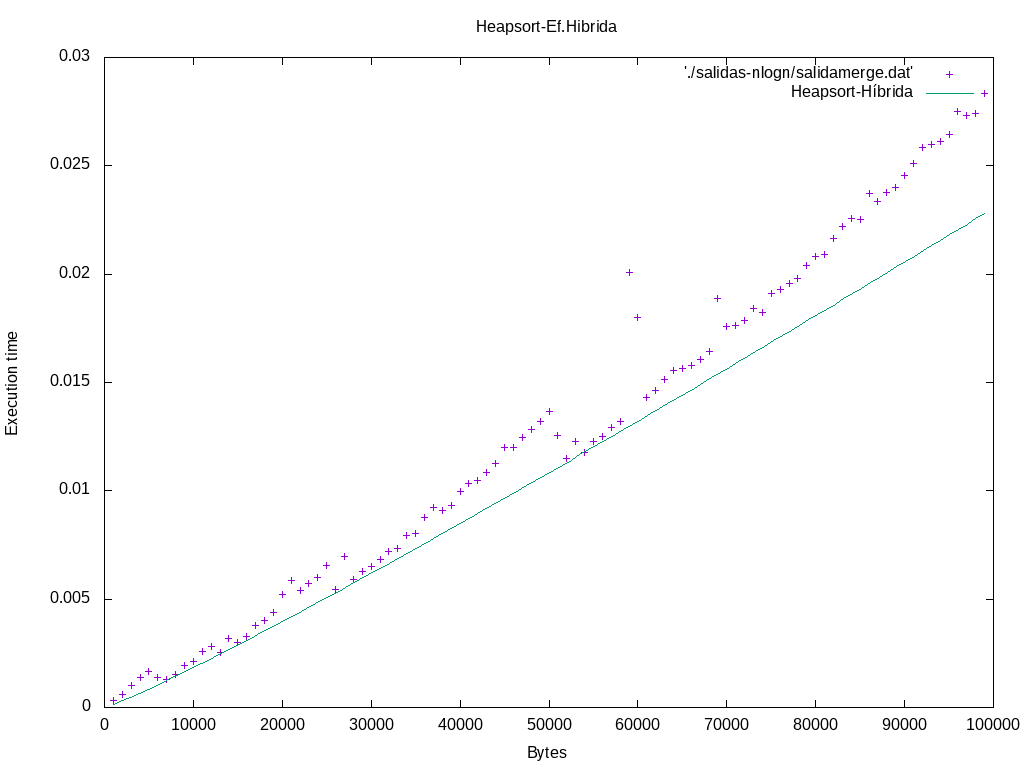
\includegraphics[scale=0.5]{imagenes/heapsort-hibrida.png}
	\caption{Heapsort, gráfica híbrida.}
	\label{fig:E12}
\end{figure}
Este algoritmo lo hemos ejecutado en otra máquina más potente, de esta manera, podemos ver como varían los tiempos de ejecución del mismo algoritmo, ejecutado en dos máquinas distintas.
\begin{itemize}
	\item Procesador (frecuencia): Intel Core i7-5500U (3.0 GHz x 2)
	\item Memoria RAM: 4 GB
	\item Disco duro: SSD 256 GB
	\item S.O: Linux Mint 17.3 Cinnamon 64-bit
\end{itemize}
El ajuste de ambas gráficas es el siguiente:
\begin{figure}[H]
	\centering
	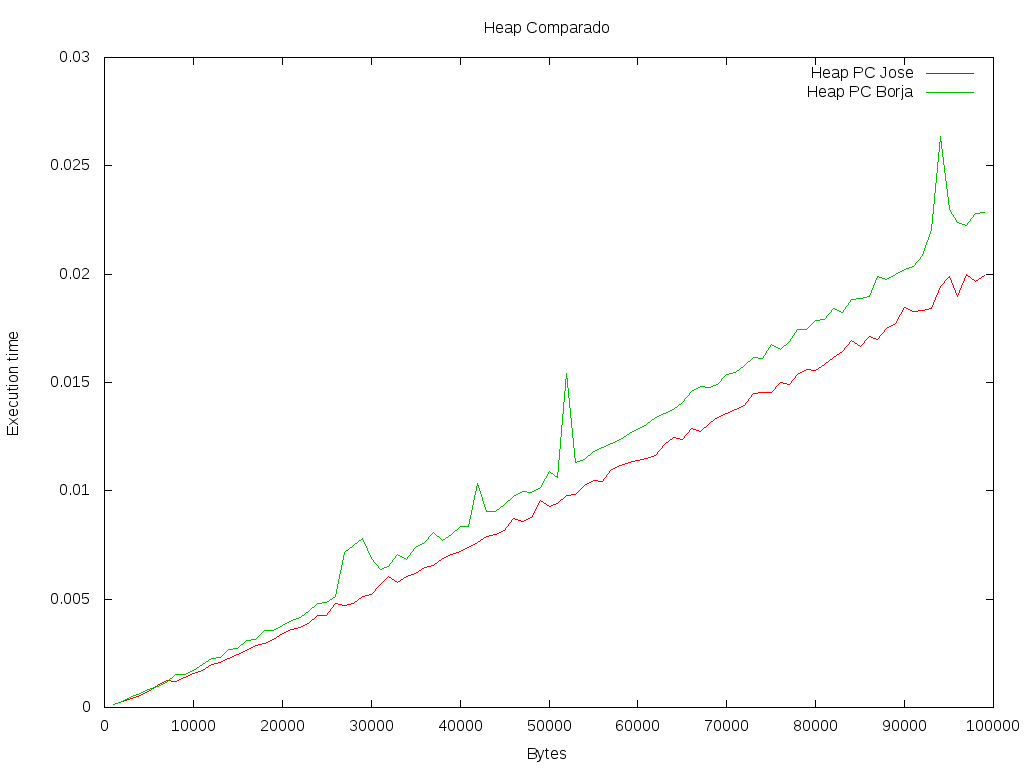
\includegraphics[scale=0.5]{imagenes/HeapComparado.png}
	\caption{Comparación en dos máquinas. Heapsort.}
	\label{fig:E13}
\end{figure}

\subsection{Merge Sort}
La gráfica empírica obtenida ha sido:
\begin{figure}[H]
	\centering
	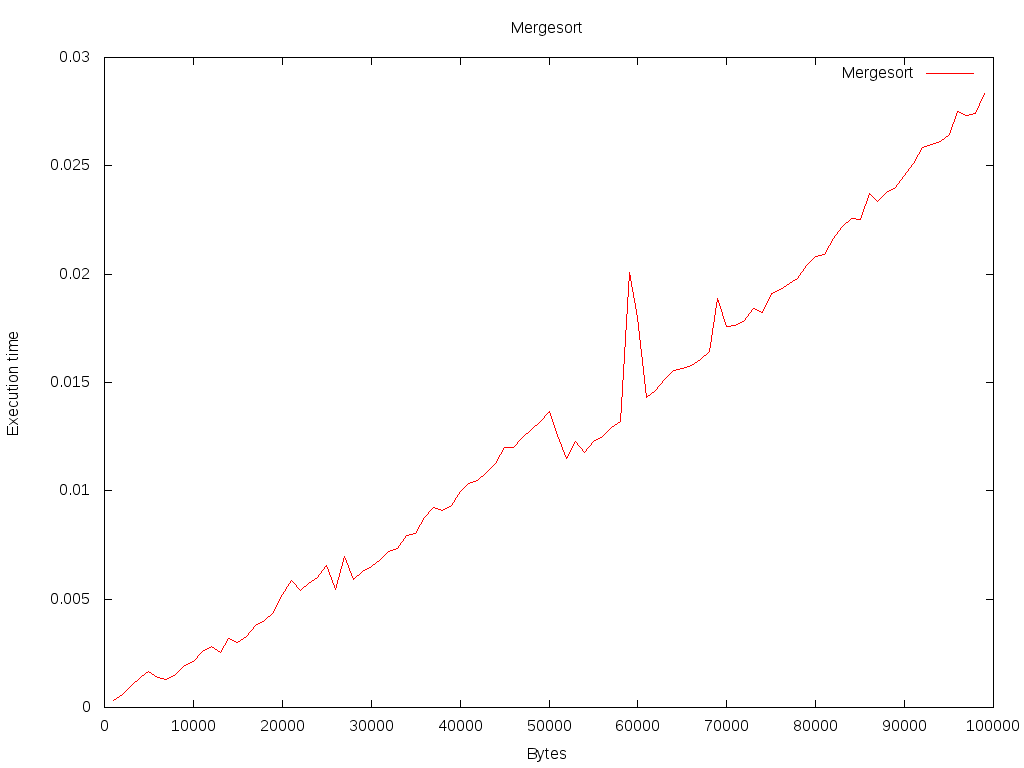
\includegraphics[scale=0.5]{imagenes/mergesort.png}
	\caption{Mergesort, gráfica empírica.}
	\label{fig:E14}
\end{figure}
La gráfica híbrida obtenida ha sido:
\begin{figure}[H]
	\centering
	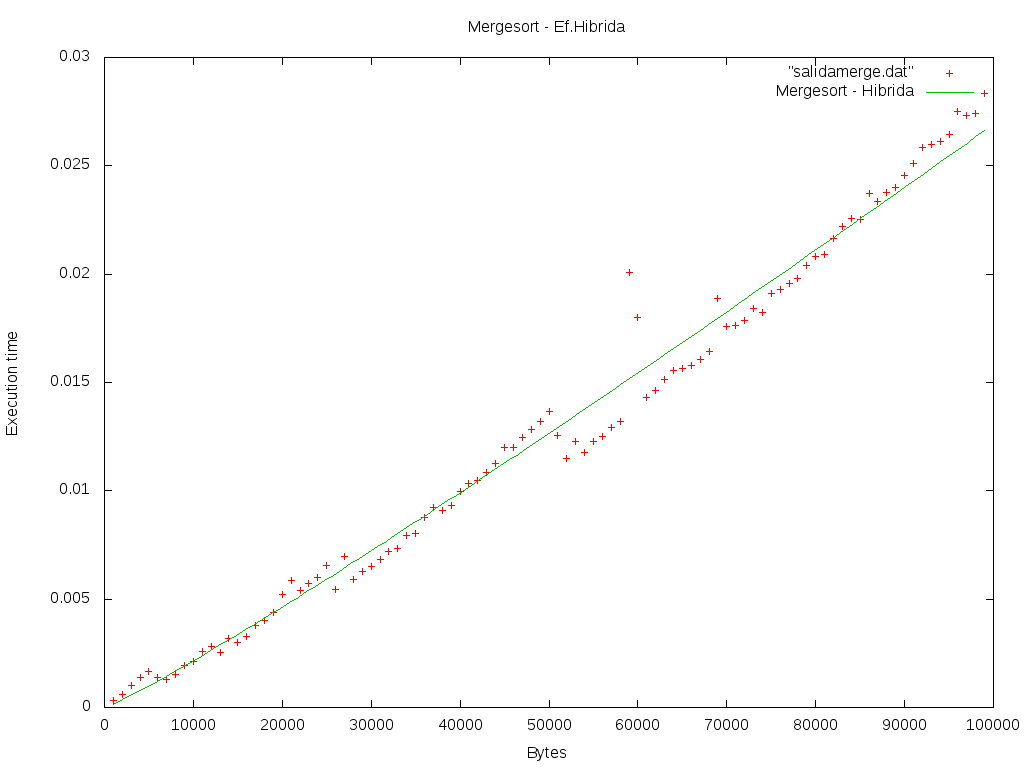
\includegraphics[scale=0.5]{imagenes/mergesort-hibrida.png}
	\caption{Mergesort, gráfica híbrida.}
	\label{fig:E15}
\end{figure}
Por último, mostramos el porcentaje de error así como las constantes ocultas.\\
\begin{center}
	\begin{tabular}{| l | c | r |}
		\hline
		\textbf{Algoritmo} & \textbf{Constante Oculta} & \textbf{Error} \\ \hline
		Mergesort & a0 = 2.33821e-08 & +/- 1.564e-10 (0.6689\%)\\ \hline
		Quicksort & a0 = 1.43368e-08 & +/- 7.621e-11 (0.5315\%) \\ \hline
		Heapsort & a0 = 2.00227e-08 & +/- 1.222e-10    (0.6104\%) \\ \hline
	\end{tabular}
\end{center}

\section{Floyd}

El algoritmo de Floyd, a diferencia de los anteriores, no es un algoritmo de ordenación. Su función, es la de encontrar el camino mínimo en grafos. La eficiencia teórica de este algoritmo es $O(n^3)$. Además de analizar la eficiencia empírica e híbrida, hemos realizado un ajuste erróneo, para demostrar que efectivamente la eficiencia de este algoritmo es la anteriormente mencionada.

\subsection{Gráficas}
\textbf{Gráfica Empírica}\\
\\
La gráfica empírica obtenida ha sido:
\begin{figure}[H]
	\centering
	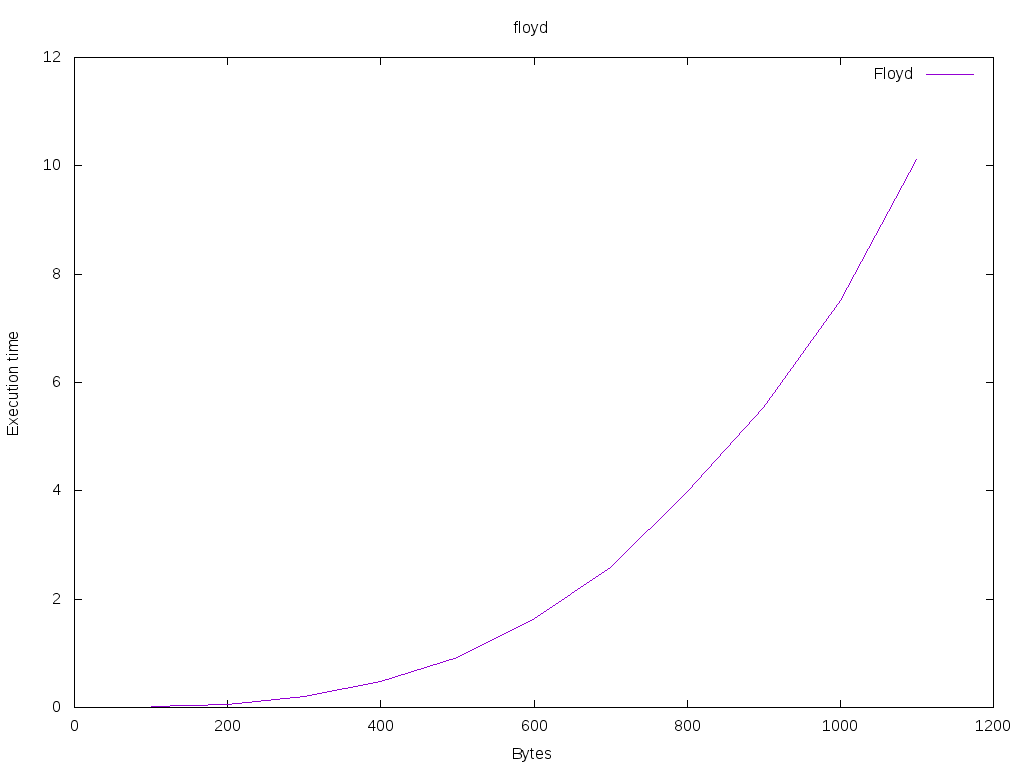
\includegraphics[scale=0.5]{imagenes/floyd.png}
	\caption{Floyd, gráfica empírica.}
	\label{fig:E16}
\end{figure}



\textbf{Gráfica Híbrida}\\
\\
La gráfica híbrida obtenida ha sido:
\begin{figure}[H]
	\centering
	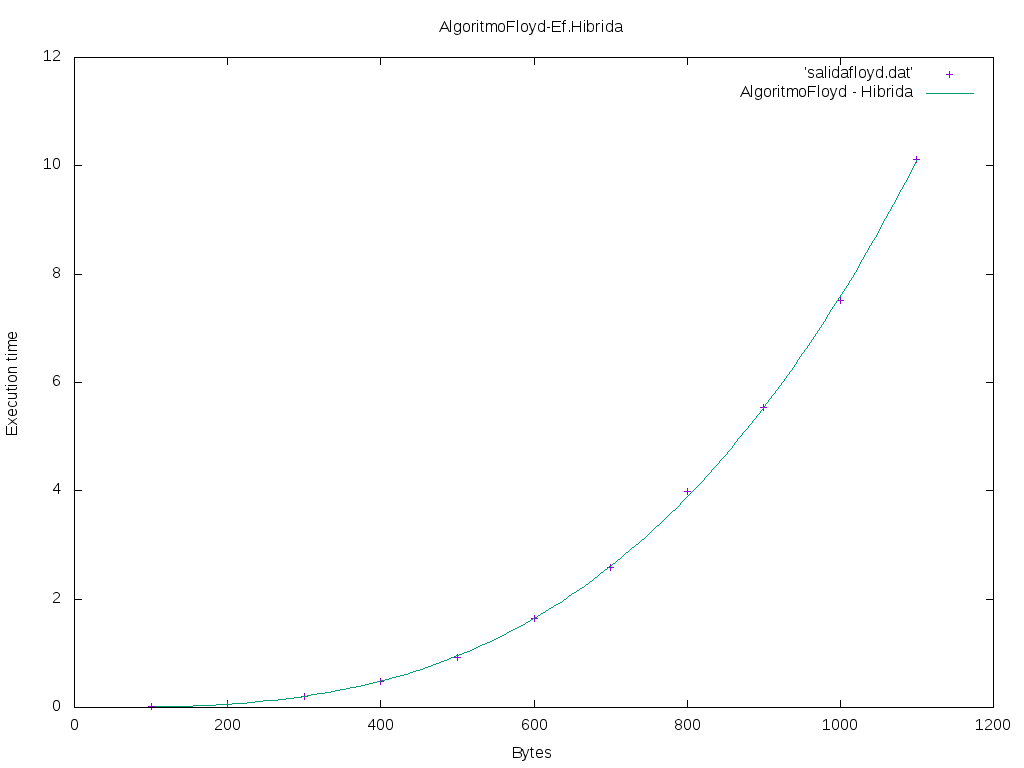
\includegraphics[scale=0.5]{imagenes/algoritmoFloyd-hibrida.png}
	\caption{Floyd, gráfica híbrida.}
	\label{fig:E17}
\end{figure}


\textbf{Ajuste Híbrido Erróneo}\\
\\

Ajuste híbrido erróneo ($O(n^3)$ ajustada a una función $O(n * log(n))$.
\begin{figure}[H]
	\centering
	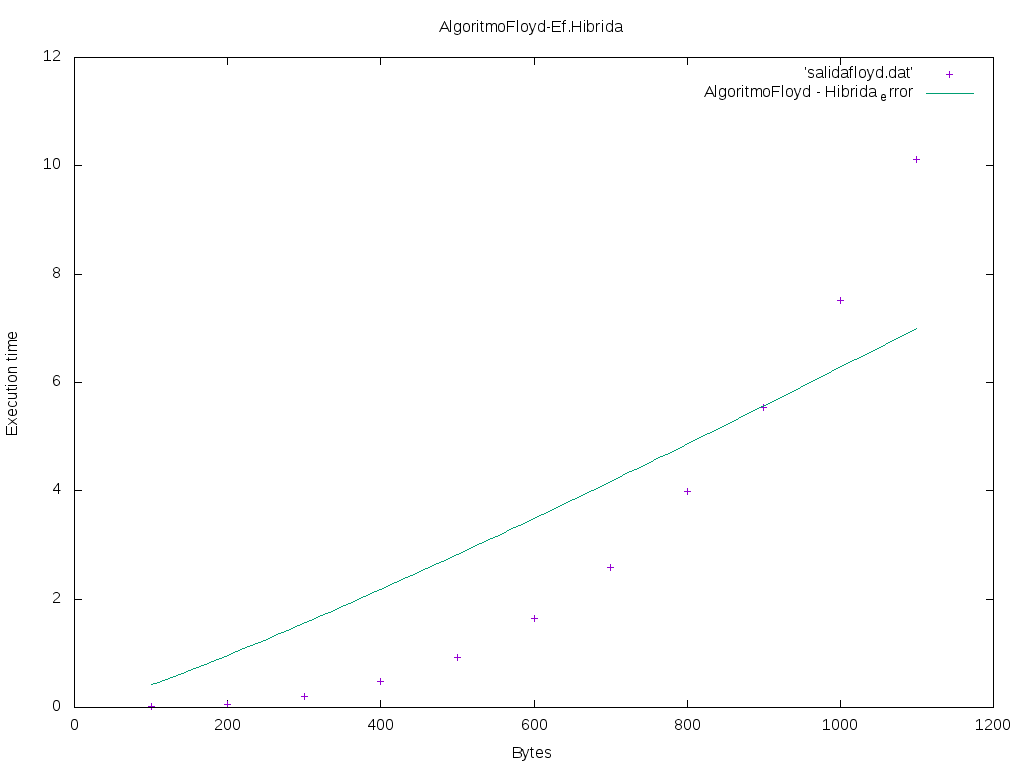
\includegraphics[scale=0.5]{imagenes/FloydError.png}
	\caption{Floyd, ajuste erróneo.}
	\label{fig:E18}
\end{figure}


\subsection{Porcentaje de error y constantes ocultas}
Por último, mostramos el porcentaje de error así como las constantes ocultas de ambos ajustes.\\

\begin{center}
	\begin{tabular}{| l | c | r |}
		\hline
		\textbf{Algoritmo} & \textbf{Constante Oculta} & \textbf{Error} \\ \hline
		Floyd & a0 = 7.59068e-09 & +/- 2.163e-11    (0.2849\%)\\ \hline
		Floyd erróneo & a0 = 0.000908818 & +/- 0.0001093 (12.03\%) \\ \hline
	\end{tabular}
\end{center}



\section{Hanoi}

El algoritmo de Hanoi, se encarga específicamente de resolver el problema de las torres de Hanoi. Este algoritmo presenta una eficiencia teórica de $O(2^n)$, lo que hace que el número de entradas para este algoritmo sea muy reducido.

\subsection{Gráficas}
La gráfica empírica obtenida ha sido:
\begin{figure}[H]
	\centering
	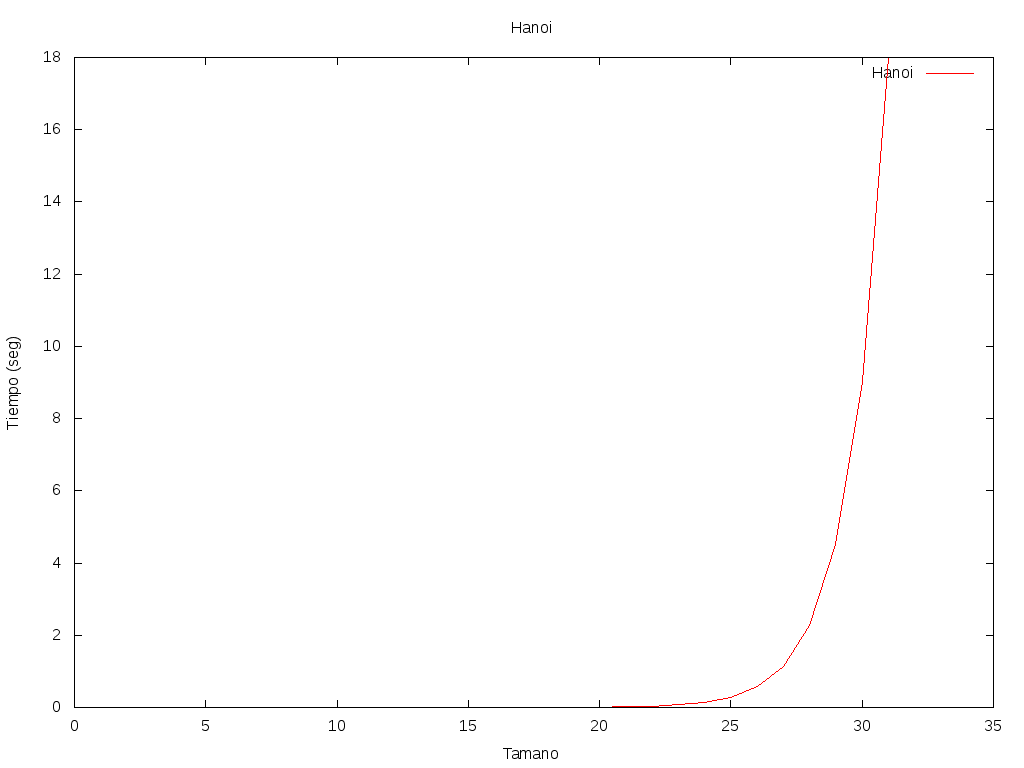
\includegraphics[scale=0.5]{imagenes/hanoiLines.png}
	\caption{Hanoi, gráfica empírica.}
	\label{fig:E19}
\end{figure}

La gráfica híbrida obtenida ha sido:
\begin{figure}[H]
	\centering
	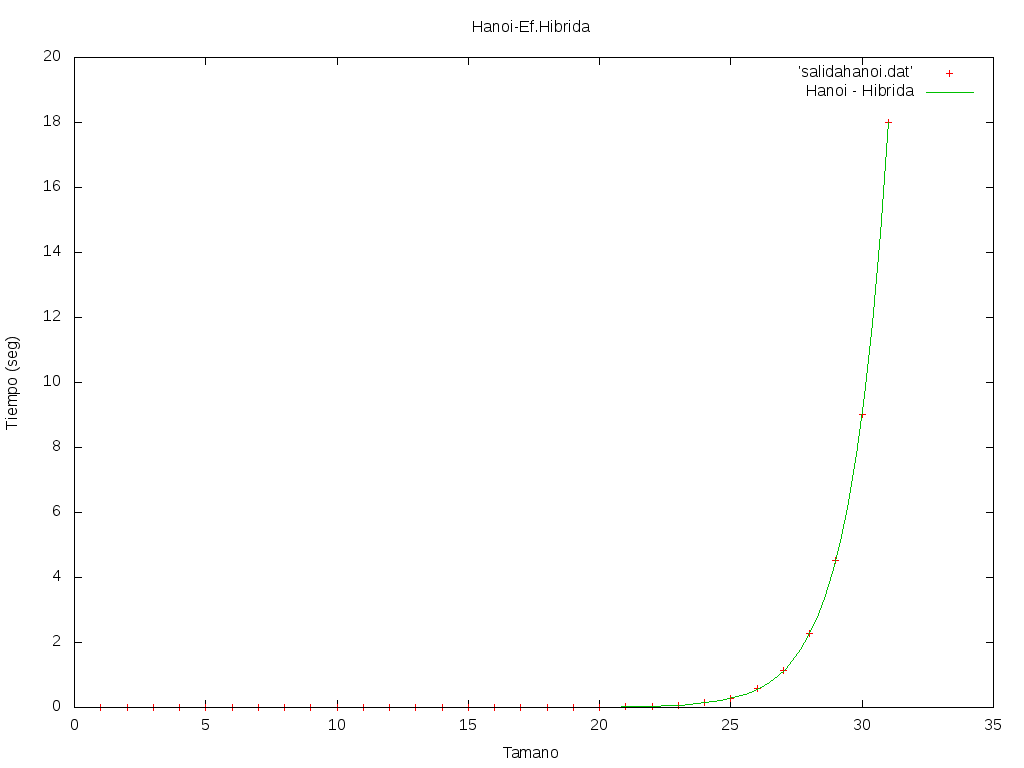
\includegraphics[scale=0.5]{imagenes/hanoi-hibrido.png}
	\caption{Hanoi, gráfica híbrida.}
	\label{fig:E20}
\end{figure}



\subsection{Comparaciones}
En este algoritmo hemos hecho varias comparaciones:
\begin{itemize}
	\item Usando diferentes optimizaciones a la hora de compilar.
	\item Utilizando un lenguaje de programación distinto (Python vs C++).
\end{itemize}

\subsection{Hanoi en Python}
La gráfica híbrida de la ejecución en Python frente a la ejecución en C++ es:
\begin{figure}[H]
	\centering
	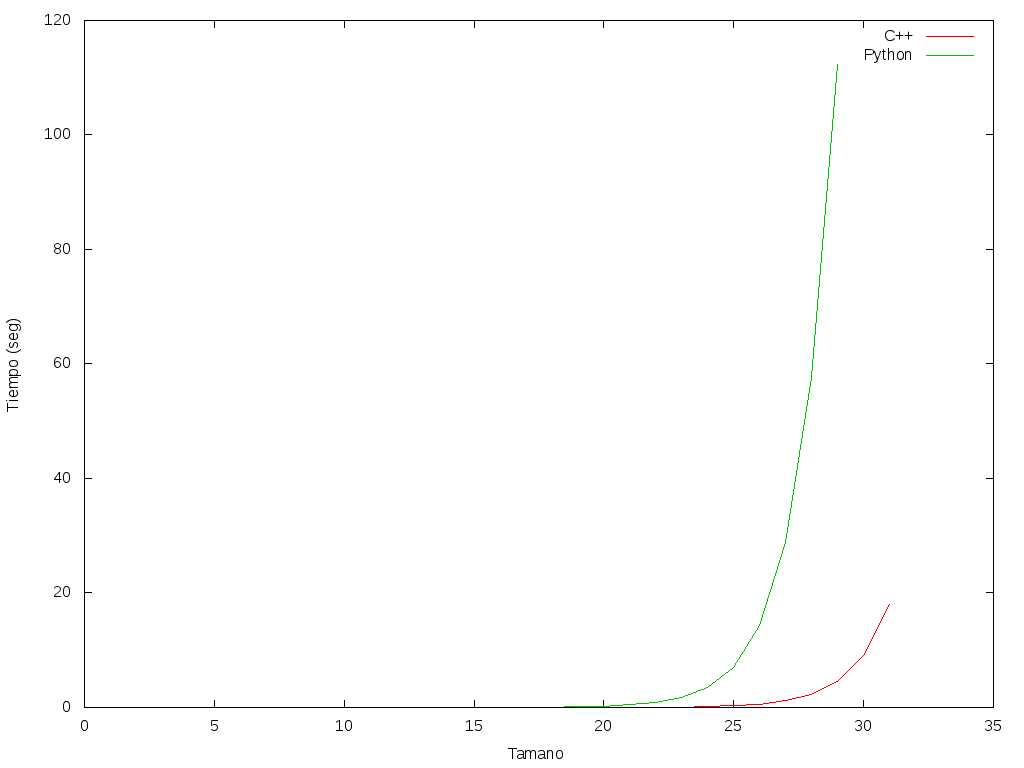
\includegraphics[scale=0.5]{imagenes/HanoiPy.png}
	\caption{Hanoi, Python - C++}
	\label{fig:E21}
\end{figure}



\subsection{Hanoi con diferentes optimizaciones}
A continuación mostramos una gráfica con los tiempos del algoritmo en función de su optimización:
\begin{figure}[H]
	\centering
	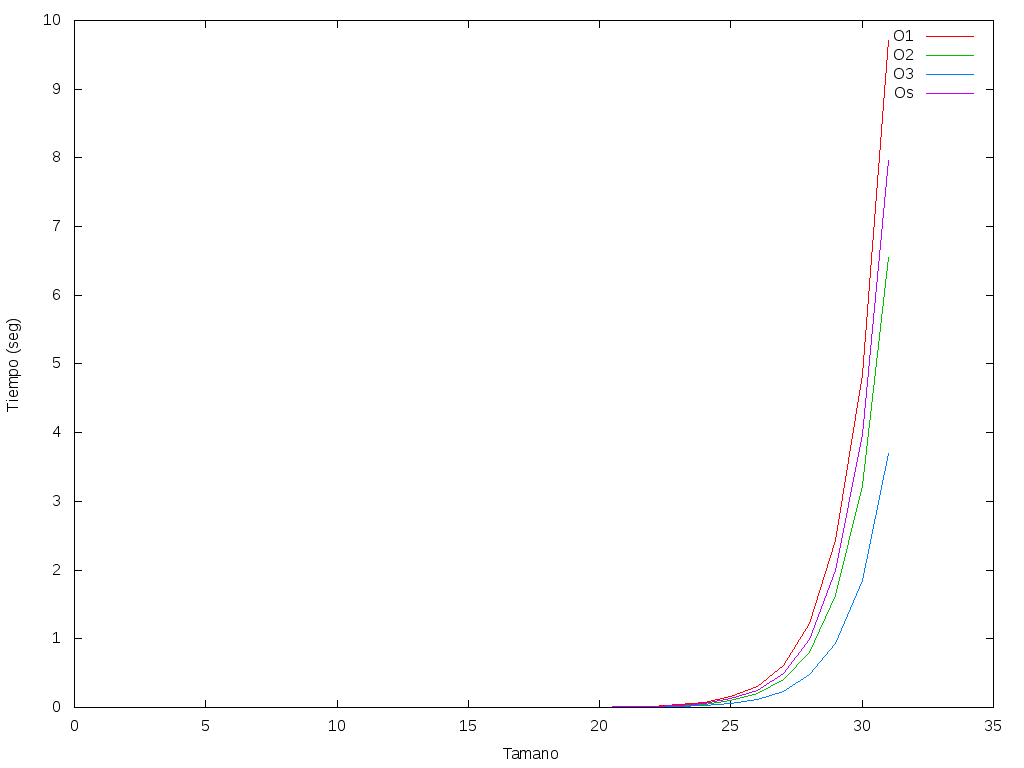
\includegraphics[scale=0.5]{imagenes/HanoiComparacion.png}
	\caption{Hanoi, gráfica con diferentes eficiencias.}
	\label{fig:E22}
\end{figure}



\subsection{Porcentaje de error y constantes ocultas}
Por último, mostramos el porcentaje de error así como las constantes ocultas.\\
\begin{center}
	\begin{tabular}{| l | c | r |}
		\hline
		\textbf{Algoritmo} & \textbf{Constante Oculta} & \textbf{Error} \\ \hline
		Hanoi & a0 = 8.38461e-09 & +/- 3.095e-12    (0.03691\%)\\ \hline
	\end{tabular}
\end{center}


%----------------------------------------------------------------------------------------

\end{document}